\subsection{Requirements Technology Baseline}
Questa macrofase è suddivisa in tre fasi:
\begin{itemize}
    \item \textbf{Baseline documentale} dal 2022-04-19 al 2022-05-02;
    \item \textbf{Baseline dei requisiti} dal 2022-05-03 al 2022-05-09;
    \item \textbf{Baseline delle tecnologie} dal 2022-05-10 al 2022-05-23.
\end{itemize}

\subsubsection{Baseline documentale}
\begin{itemize}
    \item \textbf{Norme di Progetto:} l'amministratore redige le norme e gli strumenti necessari ad una buona organizzazione e realizzazione del progetto;
    \item \textbf{Piano di Progetto:} l'analista rileva i possibili rischi che possono sorgere durante il progetto, il responsabile pianifica la macrofase RTB;
    \item \textbf{Piano di Qualifica:} l'analista stabilisce e redige i parametri di qualità stabilendo soglie minime accettabili e soglie desiderate; 
    \item \textbf{Verifica:} il verificatore controlla che siano state rispettate le norme e verifica il materiale scritto durante questa fase;
    \item \textbf{Checkpoint:} per la descrizione dettagliata si veda \$4.1.2 . 
\end{itemize}

\subsubsection{Baseline dei requisiti}
\begin{itemize}
    \item \textbf{Analisi dei Requisiti:} l'analista studia e descrive tutti i requisiti del progetto commissionato dal proponente, 
                comprese tutte le richieste opzionali e desiderabili (indipendentemente dalla possibilità di realizzarle tutte);
    \item \textbf{Norme di Progetto, Piano di Progetto, Piano di Qualifica:} documenti che vengono incrementati e aggiornati;
    \item \textbf{Verifica:} il verificatore controlla che siano state rispettate le norme e verifica il materiale scritto prodotto durante questa fase;
    \item \textbf{Checkpoint:} per la descrizione dettagliata si veda \$4.1.2 .
\end{itemize}

\subsubsection{Baseline delle tecnologie}
\begin{itemize}
    \item \textbf{Studio delle tecnologie:} il progettista, analizzando lati positivi e negativi, sceglie le tecnologie per il progetto, assegnando poi lo studio autonomo al gruppo.
    \item \textbf{Proof of Concept:} il progettista e il programmatore implementano la dimostrazione del progetto integrando le varie tecnologie e alcune funzionalità basilari.
    \item \textbf{Norme di Progetto, Piano di Progetto, Piano di Qualifica:} documenti che vengono incrementati e aggiornati;
    \item \textbf{Verifica:} il verificatore controlla che siano state rispettate le norme e verifica il materiale scritto e il prodotto realizzato durante questa fase;
    \item \textbf{Approvazione:} il responsabile controlla, approva il materiale e il prodotto realizzato durante questa macrofase RTB;
    \item \textbf{Checkpoint:} per la descrizione dettagliata si veda \$4.1.2;
    \item \textbf{Presentazione RTB:} viene preparata la presentazione per il colloquio e pubblicato il materiale nella repository pubblica.
\end{itemize}


\begin{landscape}
	\begin{figure}
	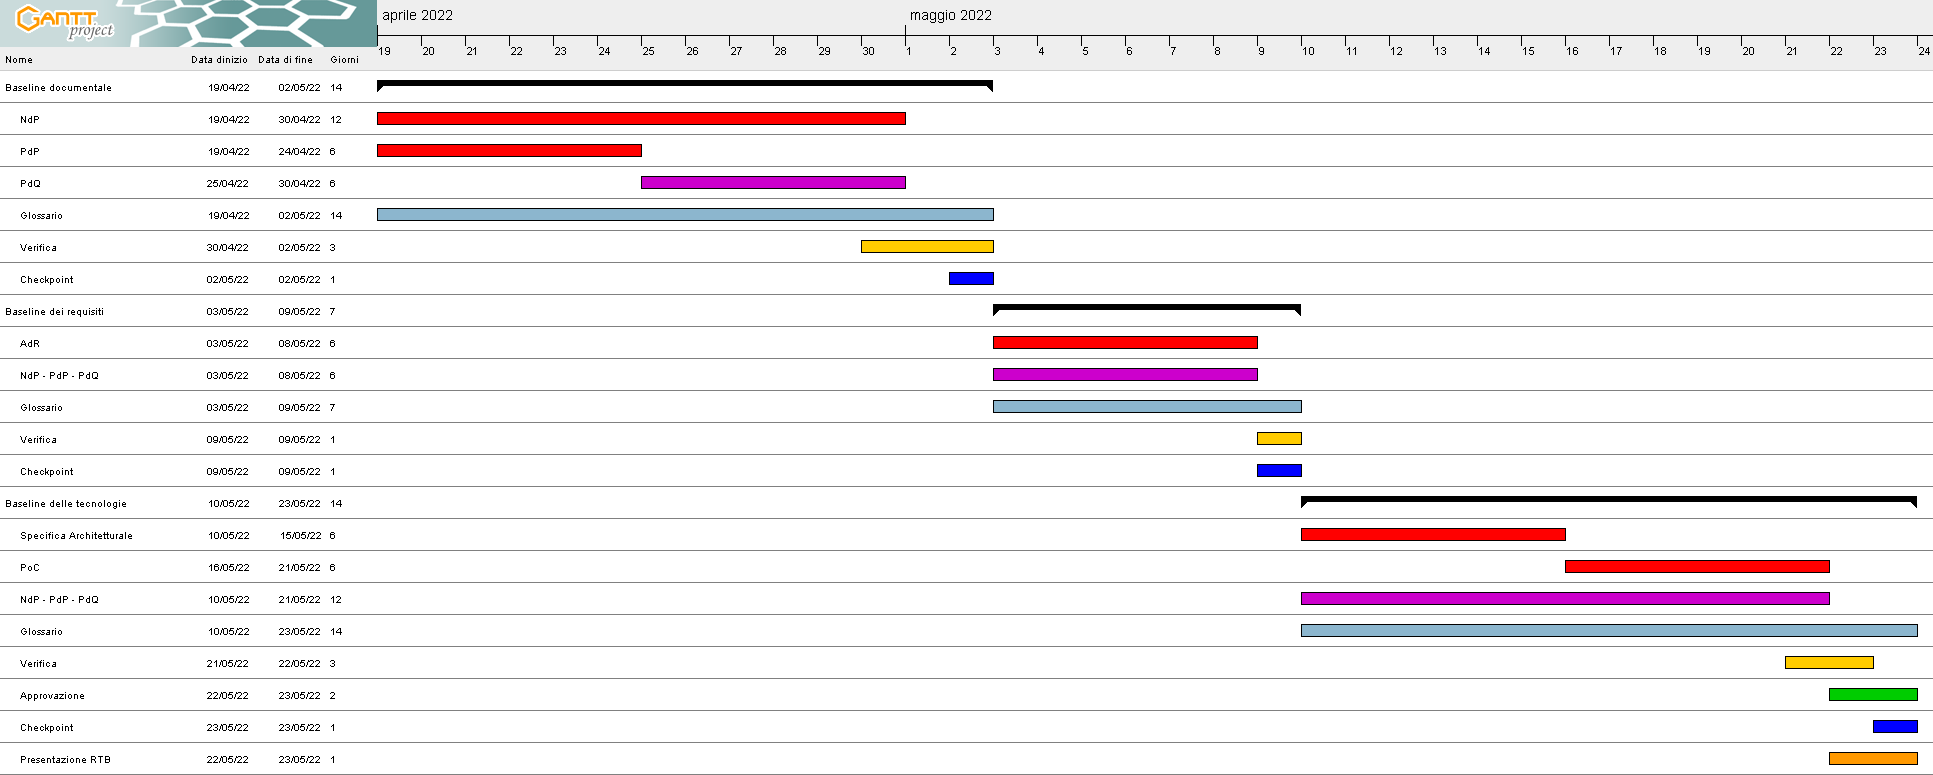
\includegraphics[width=\linewidth]{images/RTB.png}
    \caption{Diagramma di Gantt - Macrofase RTB}
	\end{figure}
\end{landscape}